\subsection{Thermal Expansion} \label{sec42}

To assess the effects of thermal expansion (TE) modeling on MC coupled multi-physics reactor simulations, a series of test problems were developed. These test problems include assembly and core problems, as well as depletion problems with restart cases. The problem geometries and material compositions were adopted from the Virtual Environment for Reactor Applications (VERA) core physics benchmark \cite{godfrey}. Additionally, ENDF/B-VII.1 was used for the MCS cross section library.

In all problems considered in this subsection, the TH parameters are updated every 500 cycles of MCS particle tracking. In MCS, the fuel pellets are axially discretized into 25 equidistant cells without radial discretization, where fission power is tallied. While the TH solvers discretize the problem axially into 25 equidistant meshes corresponding to the MCS cells. Additionally, in the TH solvers, the fuel pellets are radially discretized into 10 equidistant rings, while the cladding and gap are each represented by a single ring to numerically solve the heat conduction equation.


\subsubsection{Small Lattice Problem}

This small lattice problem consists of a $2\times2$ pin cells with two different fuel enrichments: 3.1\% wt. fuel enrichment in all fuel pins, except for the bottom-left pin, which has 2.1\% wt. enrichment, as shown in Figure \ref{fig_42a}. The pin geometry and material compositions are based on the VERA benchmark, with a 0.4 cm inter-lattice gap. The boron concentration diluted in the coolant is 1300 ppm. This problem simulated $4\times10^4$ particles per cycle, with a total of 14,500 cycles, of which 2,500 were designated as active cycles.

\begin{figure}[h]
    \centering
    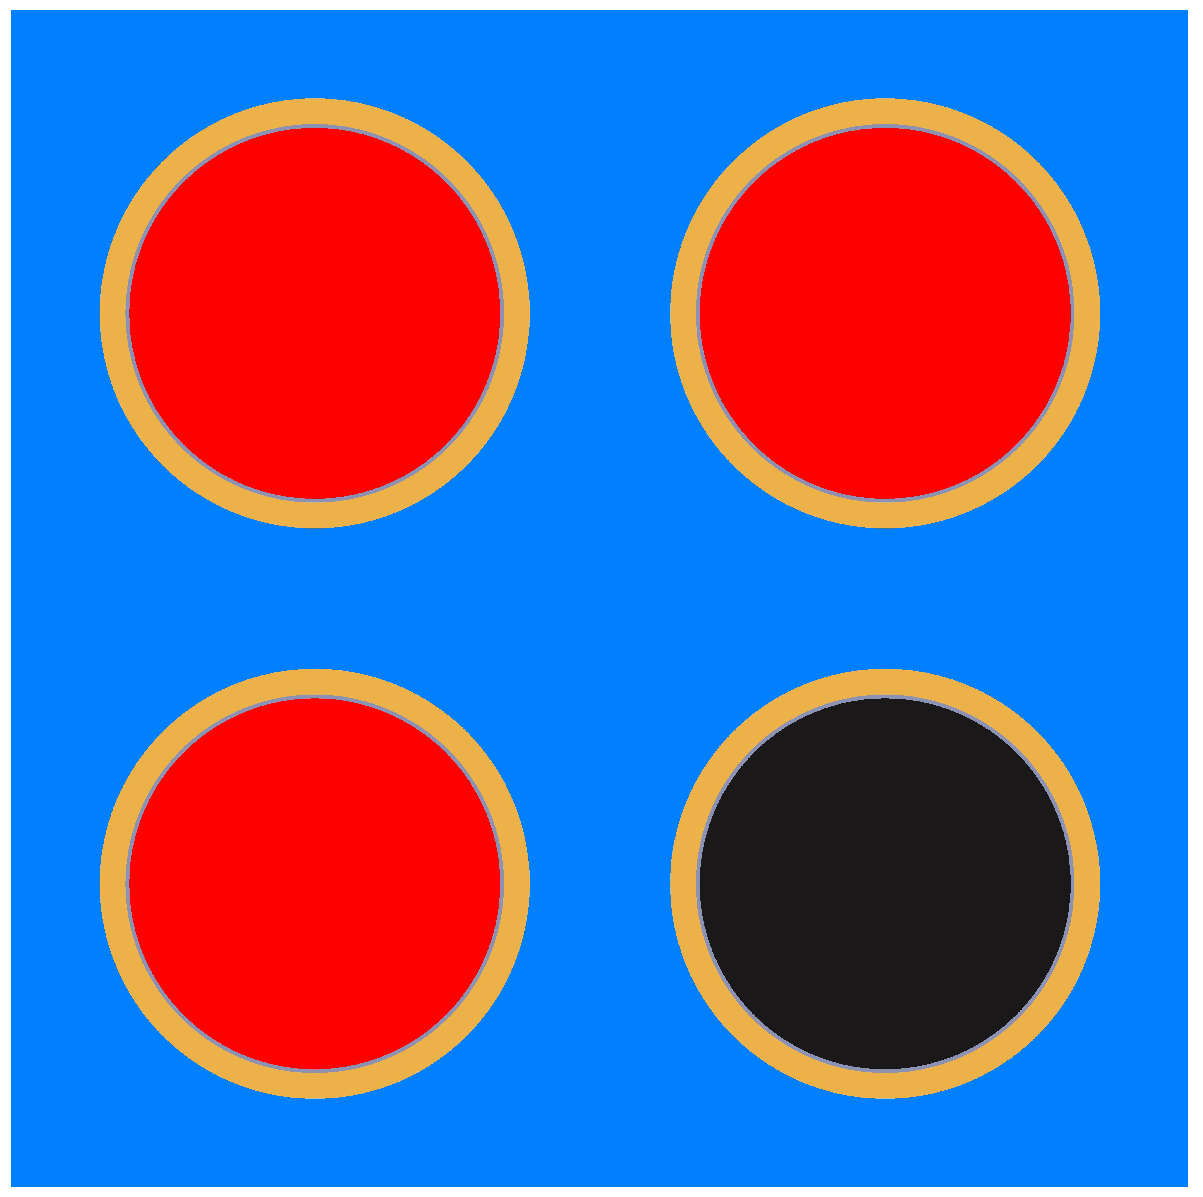
\includegraphics[width=0.4\textwidth]{figs/xy_plot_noGrid.pdf}
    \caption{Small lattice problem geometry.}
    \label{fig_42a}
\end{figure}

This simple problem is designed to evaluate the implementation of TE in the MC code MCS by comparing the solutions from on-the-fly TE in MCS to those from manually calculated TE. In the manual calculations, the geometrical expansions and expanded material densities were manually computed based on the pin-averaged temperatures from the on-the-fly thermal expansion calculation results. Note that the varying fuel enrichments in this problem result in non-uniform pin-averaged temperatures. A new MCS input file was then created using these manually calculated geometrical expansions and expanded material densities to include the equivalent TE.

Table \ref{tab42a} presents the results for small lattice problem. As observed, the on-the-fly TE and manually calculated TE produce very similar infinite multiplication factors, with only a 7 pcm difference, which is well within the given statistical uncertainty. For comparison, the result without TE is also given that shows a difference of more than 80 pcm compared to the TE cases. These results confirm that on-the-fly TE is correctly implemented in the MCS code.

\begin{table}
    \centering
    \caption{Small lattice problems infinite multiplication factors.}
    \label{tab42a} 
    % \begin{adjustbox}{width=0.6\textwidth} % Adjust your table to the text width
    \begin{tabular}{| c | c |}
    \hline 
     Cases & Reactivity differences (pcm) \\
     \hline
     On-the-fly TE          & $1.14279\pm0.00003$     \\ \hline
     Manually calculated TE & $1.14272\pm0.00004$    \\ \hline
     No TE                  & $1.14364\pm0.00003$    \\ \hline
    \end{tabular}
    % \end{adjustbox}
\end{table}


\subsubsection{Assembly Problem}

This test problem aims to assess the effects of TE at the assembly level. It is based on a case similar to Problem 6 of the VERA benchmark. The problem geometry includes non-fuel structural components such as the pin plenum, nozzles, core plates, and top and bottom reflectors. The TE effects are analyzed for various boron concentrations and fuel enrichment levels, with the reactor set to Hot Full Power (HFP) conditions. Note that the calculations for this problem simulated $4\times10^4$ particles per cycle, with a total of 14,500 cycles, of which 2,500 cycles were designated as active.

Tables \ref{tab421} and \ref{tab422} present the assembly reactivity differences caused by TE for varying boron concentrations and fuel enrichment levels, respectively. Table \ref{tab421} demonstrates that as boron concentration increases, the reactivity difference decreases. This occurs because the moderator volume, which contains boron, expands due to an increase in pin pitch. With higher boron concentrations, the neutron absorption rate rises, resulting in a lower eigenvalue. Conversely, at lower boron concentrations, the improvement in neutron moderation offsets the increase in absorption rates and yielding a higher eigenvalue. It is well known that reactivity differences due to TE are strongly influenced by boron concentration in the reactor. Similarly, Table \ref{tab422} shows that higher fuel enrichment levels lead to more positive reactivity differences due to TE. These trends in reactivity differences for varying boron concentrations and fuel temperatures are consistent with those observed in reference \cite{palmtag}.

\begin{table}
    \centering
    \caption[Assembly reactivity differences for various boron concentrations]{Assembly reactivity differences due to TE (TE - no TE) for various boron concentrations using 3.1\% wt. enriched fuel.}
    \label{tab421} 
    % \begin{adjustbox}{width=0.6\textwidth} % Adjust your table to the text width
    \begin{tabular}{| c | c |}
    \hline 
     Boron concentration (ppm) & Reactivity differences (pcm) \\
     \hline
     0        & $182\pm6$     \\ \hline
     600      & $43\pm5$     \\ \hline
     1300     & $-76\pm6$    \\ \hline
    \end{tabular}
    % \end{adjustbox}
\end{table}

\begin{table}
    \centering
    \caption[Assembly reactivity differences for different fuel enrichments]{Assembly reactivity differences due to TE (TE - no TE) for different fuel enrichment levels at a boron concentration of 600 ppm.}
    \label{tab422} 
    % \begin{adjustbox}{width=0.6\textwidth} % Adjust your table to the text width
    \begin{tabular}{| c | c |}
    \hline 
    Fuel enrichment (\% wt.) & Reactivity differences (pcm) \\
     \hline
     0        & $-35\pm4$    \\ \hline
     600      & $43\pm5$     \\ \hline
     1300     & $101\pm6$    \\ \hline
    \end{tabular}
    % \end{adjustbox}
\end{table}

\subsubsection{Whole-core Reactor Problem}

The core problem specifications are similar to those of Problem 7 from the VERA benchmark; however, instead of determining the critical boron concentration, this problem calculates eigenvalues using a fixed boron concentration of 860 ppm. The reactor operating condition is set at HFP.

\begin{table}
    \centering
    \caption{Whole-core problem eigenvalues and pin-power power errors.}
    \label{tab423} 
    \begin{adjustbox}{width=1.0\textwidth} % Adjust your table to the text width
    \begin{tabular}{| c | c | c | c | c |}
    \hline 
    Cases & Eigenvalue & Min. pin error (\%)  & Max. pin error (\%)  & RMS pin error (\%) \\
     \hline
     No TE                & $1.00046 \pm 0.00002$ & $-4.8$ & $1.9$ & $0.8$    \\ \hline
     Core-averaged        & $1.00004 \pm 0.00002$ & $-2.1$ & $1.8$ & $0.5$    \\ \hline
     Assembly-averaged    & $1.00001 \pm 0.00002$ & $-1.4$ & $2.0$ & $0.3$    \\ \hline
     Pin-averaged         & $0.99997 \pm 0.00002$ & Ref    & Ref   & Ref      \\ \hline
    \end{tabular}
    \end{adjustbox}
\end{table}

The effects of TE on the core problem are evaluated at various expansion temperatures, as can be seen in Table \ref{tab423}. For the core-averaged case, the nominal core-averaged reactor temperature at HFP is applied, with fuel expansion set at 900 K and coolant and cladding expansion at 583 K. The assembly-averaged case uses assembly-level averaged temperatures for geometry expansion within each assembly, while the pin-averaged case applies pin-level averaged temperatures for each pin cell. All cases simulated $3\times10^5$ particles per cycle over a total of 42,000 cycles, with 38,000 active cycles, resulting in a maximum relative standard deviation of 0.8\% for radial pin powers.

Table \ref{tab423} compiles the results of the whole-core reactor problem. Pin-power errors were calculated relative to the pin-averaged case. As shown in the table, when thermal expansion is not considered, the eigenvalue is overestimated compared to the pin-averaged case, and the errors at the pin level are more pronounced. Using core-averaged nominal temperatures improves the eigenvalue, reducing the difference to less than 10 pcm compared to the pin-wise case and also lowering pin-power errors. Greater accuracy is achieved when assembly-level temperatures are used for geometry expansion, yielding only a 4 pcm eigenvalue difference and a 0.3\% RMS pin error. The results indicate that as the spatial resolution of expansion temperatures increases, both the eigenvalue and pin powers converge toward those of the pin-wise case.

\begin{figure}
    \centering
    \begin{subfigure}[b]{0.5\textwidth}
        \centering
        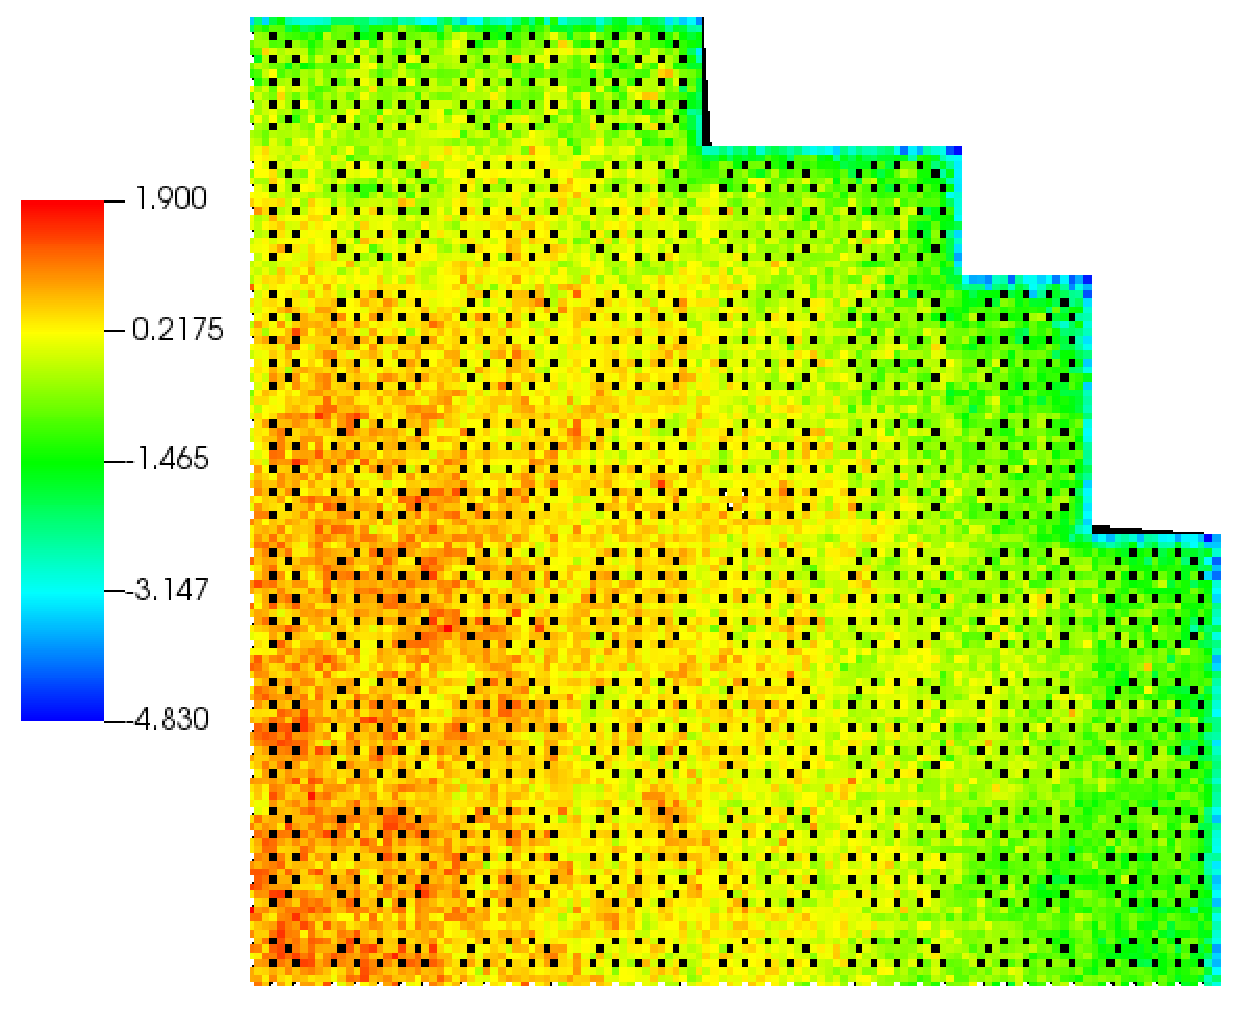
\includegraphics[width=\textwidth]{figs/pin_error_no_exp.pdf}
        \caption{No TE case}
    \end{subfigure}
    \begin{subfigure}[b]{0.5\textwidth}
        \centering
        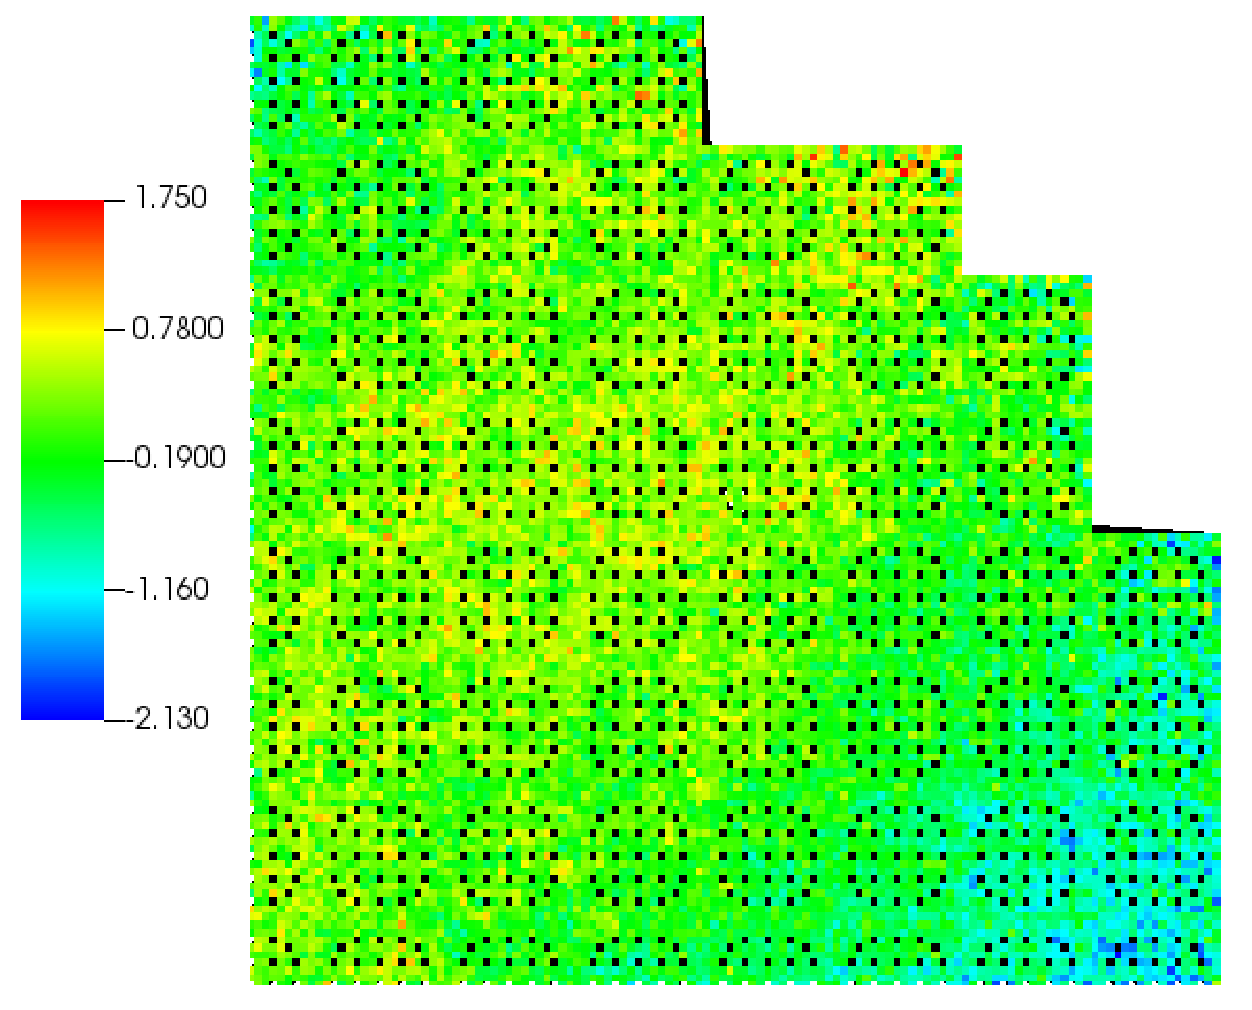
\includegraphics[width=\textwidth]{figs/pin_error_nominal.pdf}
        \caption{Core-averaged case}
    \end{subfigure}
    \begin{subfigure}[b]{0.5\textwidth}
        \centering
        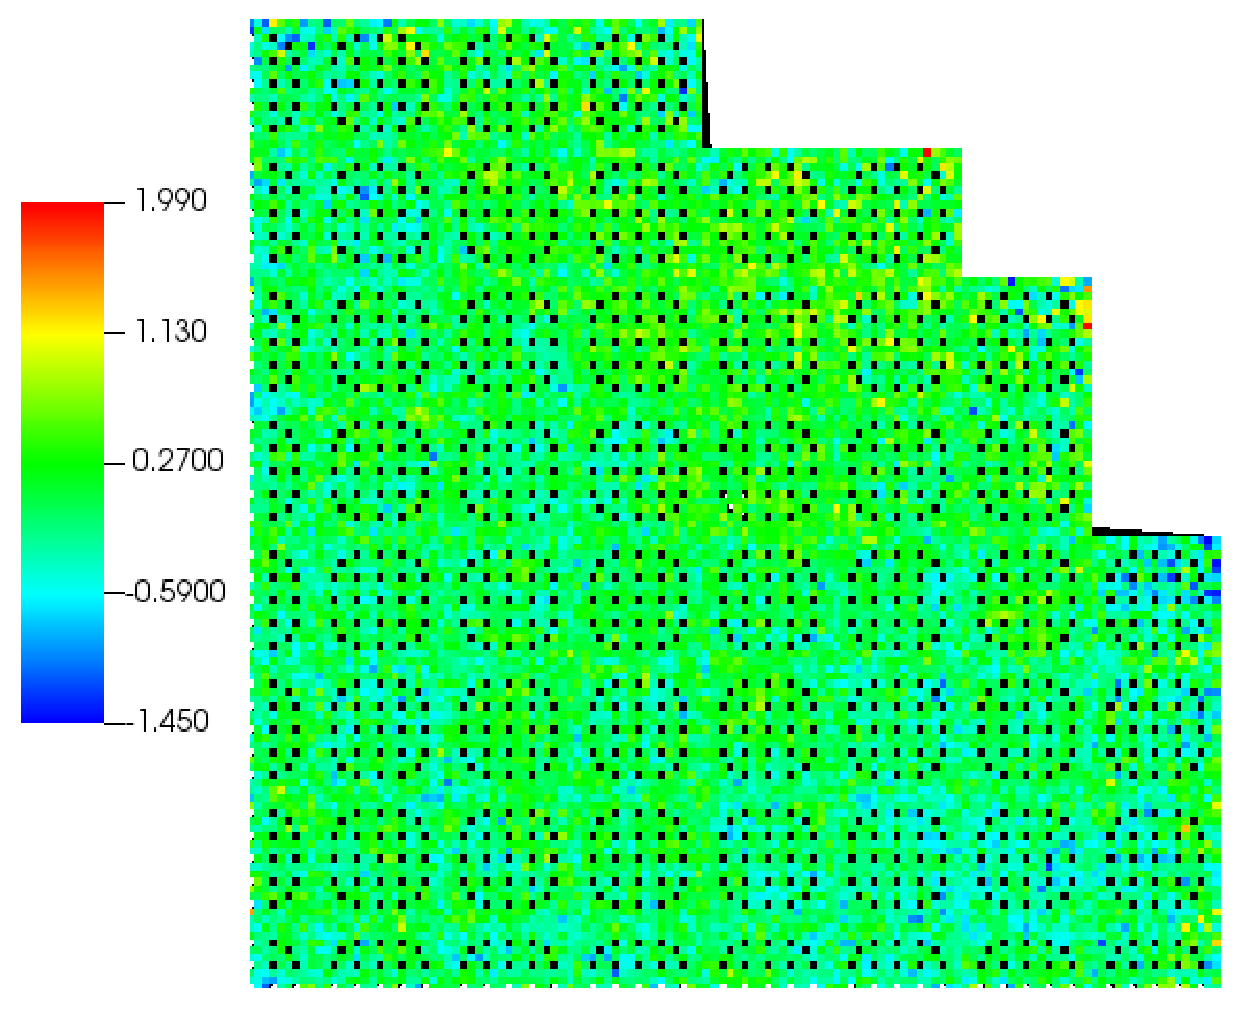
\includegraphics[width=\textwidth]{figs/pin_error_assembly.pdf}
        \caption{Assembly-averaged case}
    \end{subfigure}
    \caption[Radial pin-power errors distributions relative to the pin-averaged case]{Radial pin-power errors distributions relative to the pin-averaged for each case}
    \label{fig_421}
\end{figure}

Figure \ref{fig_421} presents the radial pin-power errors relative to the pin-averaged case. The no-TE case underestimates pin powers at the core periphery by up to -4.8\%, while overestimating pin powers near the core center. The core-averaged case yields reasonably accurate pin powers but still exhibits some deviations. The assembly-averaged case produces pin-power solutions that closely align with the pin-averaged case. Additionally, it is notable that the pin-wise case's runtime is only 0.9\% longer than the no-TE case, indicating that incorporating on-the-fly thermal expansion introduces virtually no additional computational cost.

\subsubsection{Isothermal Temperature Coefficient}

This test problems attempts to quantify the effect of thermal expansion on the isothermal temperature coefficient (ITC). The ITC represents the change in reactivity per unit change in fuel and moderator temperature \cite{ansi}. ITC measurements are typically performed during Hot Zero Power (HZP) reactor physics tests to determine whether the measured ITC aligns with the calculated value \cite{hong}.

In this study, the ITC measurement in the VERA benchmark was modeled for cases with and without TE. The reactor used in this benchmark is Watts Bar Unit 1, a Westinghouse PWR. The measured ITC was obtained during cycle 1, with all fresh fuel. The ITC was calculated using isothermal temperatures of 560 K and 570 K, with a boron concentration of 1291 ppm. 

To ensure statistical reliability, the ITC mean and the corresponding standard deviations were obtained by performing five runs for each case, with random seeds for each run. This resulted in a total of 25 ITC samples, from which the mean and standard deviation were calculated. For each run, there were 14,500 cycles, of which 2,500 cycles were inactive, with $4\times10^4$ particle histories simulated for every cycle. The results are displayed and compared against measurement result in Table \ref{tab424}.


\begin{table}
    \centering
    \caption{Calculated ITCs compared with the measured value.}
    \label{tab424} 
    % \begin{adjustbox}{width=0.6\textwidth} % Adjust your table to the text width
    \begin{tabular}{| c | c |}
    \hline 
    Cases & ITC (pcm/$^{\circ}$F) \\
     \hline
     No TE                & $-3.74 \pm 0.24 $    \\ \hline
     TE                   & $-3.31 \pm 0.22 $    \\ \hline
     Measurement          & $-2.17 $    \\ \hline
    \end{tabular}
    % \end{adjustbox}
\end{table}

As indicated in the table, incorporating TE into core modeling improves the accuracy of the ITC, bringing it closer to the measured data. Additionally, the results show that TE modeling makes the ITC more positive by 0.4 pcm/$^{\circ}$F. This difference is slightly higher than the findings in Palmtag et al. \cite{palmtag}, which reported that TE modeling increases the ITC by 0.2-0.3 pcm/$^{\circ}$F.

Although the ITC solutions for both the TE and No TE cases deviate significantly from the reported measured value, they are still comparable to the results of other MC calculations. For example, the ITC solution from KENO without TE is 3.18 pcm/$^{\circ}$F \cite{godfrey}.

\subsubsection{Whole-core Reactor Depletion using Restart Calculations}

Exercise 3 of the TVA Watts Bar Unit 1 multi-physics depletion benchmark \cite{albagami} was adopted to investigate the effect of TE on the boron letdown curve during reactor depletion. Restart cases from whole-core pin-by-pin depletion without TE were run at 0, 221.1, and 392.3 effective full power days (EFPDs) for cases with and without TE. This depletion problem simulated $6\times10^4$ particles per cycles, with a total of 5,000 cycles, of which 2,500 were active cycles.

MCS, coupled with the CTF thermal-hydraulics solver \cite{salko}, was used to solve this problem. The work on MCS/CTF multi-physics coupling was done in the previous studies \cite{yu_2017}. The results were compared against the measured values obtained from reference \cite{godfrey} and are presented in Table \ref{tab_425}.

As shown in the table, direct core modeling with TE yields more accurate predictions for this depletion whole-core problem, particularly as power increases and fuel burnup progresses. At the beginning of the cycle (BOC), core modeling with TE underestimates the measured critical boron concentration (CBC) by 22 ppm, which is slightly higher than the 13-ppm underestimation observed with core modeling without TE. This higher CBC underestimation in the TE model at BOC is attributed to the high boron concentration and zero power at the start of the cycle. However, as the fuel cycle progresses and power increases, core modeling with TE offers more precise CBC solutions. For instance, at the end of the cycle (EOC), the TE model underestimates the CBC by just 3 ppm, compared to a 27-ppm underestimation by the model without TE. These results indicate that direct core modeling with TE provides more accurate solutions, particularly at full power and higher fuel burnup levels.

\begin{table}
    \centering
    \caption{Critical boron concentrations for depletion problem.}
    \label{tab_425} 
    % \begin{adjustbox}{width=\textwidth} % Adjust your table to the text width
    \begin{tabular}{| c | c | c | c | c | c | c | }
    \hline
          &       &               &              & \multicolumn{3}{|c|}{Critical Boron Concentration (ppm)}   \\
    \cline{5-7}
     Cases & EFPDs & Percent power & Bank D step & Measurement &   TE            & No TE             \\
     \hline
     BOC    & 0.0    & 0.0           & 186         & 1299        & $1277 \pm 0.8$  &  $1286 \pm 0.6$    \\ \hline
     MOC    & 221.1  & 100.0         & 222         & 530         & $485  \pm 0.9$  &  $474  \pm 0.8$    \\ \hline
     EOC    & 392.3  & 86.9          & 202         & 38          & $35   \pm 0.9$  &  $11   \pm 0.7$    \\ \hline
    \end{tabular}
    % \end{adjustbox}
\end{table}
